\documentclass[11pt, twoside, pdftex]{article}

% This includes all of the settings that we should use for the document
\newcommand{\PDFTitle}{Using Triple-Speed Ethernet on DE2-115 Boards}
\newcommand{\commonPath}{../../../Common}
\newcommand{\datePublished}{Mar 2022}

\newcommand{\versnum}{21.1} %version number quartus/AMP
\newcommand{\quartusname}{Quartus\textsuperscript{\textregistered} Prime}	
\newcommand{\textBar}{For \quartusname{} \versnum{}}
\newcommand{\thisyear}{2022 } %for copyright
\newcommand{\company}{FPGAcademy.org}
\newcommand{\longteamname}{FPGAcademy.org}
\newcommand{\teamname}{FPGAcademy}
\newcommand{\website}{FPGAcademy.org}

\newcommand{\productAcronym}{AMP}
\newcommand{\productNameShort}{Monitor Program}

\newcommand{\productNameMedTM}{Monitor Program}
\newcommand{\productNameMed}{Monitor Program}

%\newcommand{\headerLogoFilePath}[1]{#1/FPGAcademy.png}



\setlength\topmargin{-0.25in}
\setlength\headheight{0in}
\setlength\headsep{0.35in}
\setlength\textheight{8.5in}
\setlength\textwidth{7in}
\setlength\oddsidemargin{-0.25in}
\setlength\evensidemargin{-0.25in}
\setlength\parindent{0.25in}
\setlength\parskip{0in} 

\pdfpagewidth 8.5in
\pdfpageheight 11in

% listings is a package that supports encapsulating source code in LaTeX conveniently

\usepackage{listings}
% add support for graphics
\usepackage{graphicx}
\usepackage[usenames, dvipsnames]{color}

\def\expandparam\lstinputlisting[#1]#2{\edef\tmp{\noexpand\lstinputlisting[#1]{#2}}\tmp}

\widowpenalty 10000
\clubpenalty 10000

%%%%%%%%%%%%%%%%%%%% Source Code Formatting %%%%%%%%%%%%%%%%%%%%
\definecolor{globalCommentColour}{rgb}{0.588,0.588,0.588}

%%%%%%%%%%%%%%%%%%%%%%%%%%%%%%%%%%%%%%%%%%%%%%%%%%%%
% Defining a NiosII ASM highlighter for lstlisting
\lstdefinelanguage[NiosII]{Assembler} {
 	morekeywords={add, addi, and, andhi, andi, beq, bge, bgeu, bgt, bgtu, ble,  bleu, blt, bltu, bne, br, break,% 
 	bret, call, callr, cmpeq, cmpeqi, cmpge, cmpgei, cmpgeu, cmpgeui, cmpgt, cmpgti, cmpgtu, cmpgtui, cmple,%
 	cmplei, cmpleu, cmpleui, cmplt, cmplti, cmpltu, cmpltui, cmpne, cmpnei, custom, div, divu, eret, flushd,%
 	flushda, flushi, flushp, initd, initda, initi, jmp, jmpi, ldb, ldbio, ldbu, ldbuio, ldh, ldhio, ldhu, ldhuio,%
 	ldw, ldwio, mov, movhi, movi, movia, movui, mul, muli, mulxss, mulxsu, mulxuu, nextpc, nop, nor, or, orhi, ori,%
 	rdctl, rdprs, ret, rol, roli, ror, sll, slli, sra, srai, srl, srli, stb, stbio, sth, sthio, stw, stwio,%
 	sub, subi, sync, trap, wrctl, wrtcl, wrprs, xor, xori, xorhi, xori},% 	
 	morekeywords=[2]{.abort, .ABORT, .align, .app-file, .ascii, .asciz, .balign, .byte, .comm, .data, .def,%
 	.desc, .dim, .double, .eject, .else, .end, .endef, .endif, .equ, .equiv, .err, .extern, .file, .fill, .float,%
 	.global, .globl, .hword, .ident, .if, .include, .int, .irp, .irpc, .lcomm, .lflags, .line, .linkonce, .ln,%
 	.list, .long, .macro, .mri, .nolist, .octa, .org, .p2align, .psize, .quad, .rept, .sbttl, .scl, .section,%
 	.set, .short, .single, .size, .sleb128, .skip, .space, .stadb, .stabn, .stabs, .string, .symver, .tag,%
 	.text, .title, .type, .val, .uleb128, .word},% 	
 	morekeywords=[3]{et, bt, gp, sp, fp, ea, sstatus, ra, pc, status, estatus, bstatus, ienable, ipending, cpuid,%
 	exception, pteaddr, tlbacc, tlbmisc, eccinj, badaddr, config, mpubase, mpuacc},% 	
 	sensitive=t,%
 	alsoletter=.,%
	morestring=[b]",%
 	morecomment=[s]{/*}{*/},%
 	morecomment=[l]\#,%
   }[keywords,comments,strings]
   
   %% NOTE: morekeywords=[2] are GNU directives.
   
   \definecolor{niosInstructionColour}{rgb}{0.000,0.608,0.000}
   \definecolor{niosDirectiveColour}{rgb}{0.000,0.000,0.902}
   \definecolor{niosSpecialRegColour}{rgb}{0.000,0.000,0.000}
   \definecolor{niosStringColour}{rgb}{0.808,0.482,0.000}
   
   %% NOTE: To make bold use: =\bfseries\color{<colour>}
   \lstdefinestyle{defaultNiosStyle} {
   language=[NiosII]{Assembler},
   stringstyle=\color{niosStringColour},
   keywordstyle=\color{niosInstructionColour},
   keywordstyle=[2]\color{niosDirectiveColour},
   keywordstyle=[3]\itshape\color{niosSpecialRegColour}
   }
%%%%%%%%%%%%%%%%%%%%%%%%%%%%%%%%%%%%%%%%%%%%%%%%%%%%

%%%%%%%%%%%%%%%%%%%%%%%%%%%%%%%%%%%%%%%%%%%%%%%%%%%%
% Defining a ArmA9 ASM highlighter for lstlisting
\lstdefinelanguage[ArmA9]{Assembler} {
 	morekeywords={ADC, ADD, ADDS, AND, ANDS, B, BAL, BEQ, BGE, BGT, BL, BLT, BIC, BKPT, BLX, BNE, BX, CDP, CLZ, CMN, CMP, EOR,%
 	EORS, LDC, LDM, LDR, LDRB, LDRBT, LDRH, LDRSB, LDRSH, LDRT, LSL, MCR, MLA, MOV, MOVW, MOVT, MRC, MRS, MSR, MUL, MVN, ORR, PLD,%
 	ROR, RSB, RSC, SBC, SMLAL, SMULL, STC, STM, STR, STRB, STRBT, STRH, STRT, SUB, SUBS, SWI, SWP, SWPB, TEQ, UMLAL,
 	PUSH, POP, MOVS, RORS, LSR},%
 	morekeywords=[2]{.abort, .ABORT, .align, .app-file, .ascii, .asciz, .balign, .byte, .comm, .data, .def,%
 	.desc, .dim, .double, .eject, .else, .end, .endef, .endif, .equ, .equiv, .err, .extern, .file, .fill, .float,%
 	.global, .globl, .hword, .ident, .if, .include, .int, .irp, .irpc, .lcomm, .lflags, .line, .linkonce, .ln,%
 	.list, .long, .macro, .mri, .nolist, .octa, .org, .p2align, .psize, .quad, .rept, .sbttl, .scl, .section,%
 	.set, .short, .single, .size, .sleb128, .skip, .space, .stadb, .stabn, .stabs, .string, .symver, .tag,%
 	.text, .title, .type, .val, .vectors, .uleb128, .word},%
 	morekeywords=[3]{SP, PC, MIDR, CTR, TCMTR, TLBTR, MPIDR, ID_PFR0, ID_PFR1, ID_DFR0, ID_MMFR0, ID_MMFR1, ID_MMFR2,%
 	ID_MMFR3, ID_ISAR0, ID_ISAR1, ID_ISAR2, ID_ISAR3, ID_ISAR4, CCSIDR, CLIDR, AIDR, CSSELR, TTBR0, TTRB1, TTBR2, DACR,%
 	DFSR, IFSR, ADFSR, AIFSR, DFAAR, IFAR, ICIALLUIS, BPIALLIS, PAR, ICIALLU, ICIMVAU, BPIALL, DCIMVAC, DCISW, V2PCWPR,%
 	DCCVAC, DCCSW, DDIMVAC, DCISW, TLBALLIS, TLBIMVAIS, TLBIASIDIS, TLBIMVAAIS, TLBIALL, TLBIMVA, TLBIASID, TLBIMVAA,%
 	PMCR, PMCNTENSET, PMCNTENCLR, PMOVSR, PMSWINC, PMSELR, PMXEVTYPER, PMXEVCNTR, PMUSERENR, PMINTENSET, PMINTENCLR,%
 	PRRR, NRRR, PLEIDR, PLEASR, PLEFSR, PLEUAR, PLEPCR, VBAR, MVBAR, ISR, FCSEIDR, CONTEXTIDR, TPIDRURW, TPIDRURO, TPIDRPRW},%
 	sensitive=f,%
 	alsoletter=.,%
	morestring=[b]",%
 	morecomment=[s]{/*}{*/},%
 	morecomment=[l]{//},%
   }[keywords,comments,strings]
   
   %% NOTE: morekeywords=[2] are GNU directives.
   
   \definecolor{armInstructionColour}{rgb}{0.000,0.608,0.000}
   \definecolor{armDirectiveColour}{rgb}{0.000,0.000,0.902}
   \definecolor{armSpecialRegColour}{rgb}{0.000,0.000,0.000}
   \definecolor{armStringColour}{rgb}{0.808,0.482,0.000}
   
   \lstdefinestyle{defaultArmStyle} {
   language=[ArmA9]{Assembler},
   stringstyle=\color{armStringColour},
   keywordstyle=\color{armInstructionColour},
   keywordstyle=[2]\color{armDirectiveColour},
   keywordstyle=[3]\itshape\color{armSpecialRegColour}
   }
%%%%%%%%%%%%%%%%%%%%%%%%%%%%%%%%%%%%%%%%%%%%%%%%%%%%

%%%%%%%%%%%%%%%%%%%%%%%%%%%%%%%%%%%%%%%%%%%%%%%%%%%%
% Defining style for the verilog.

\definecolor{verilogCommentColour}{rgb}{0.000,0.502,0.000}

\lstdefinestyle{defaultVerilogStyle} {
language={Verilog},
keywordstyle=\color{blue},
commentstyle=\color{verilogCommentColour}
}
%%%%%%%%%%%%%%%%%%%%%%%%%%%%%%%%%%%%%%%%%%%%%%%%%%%%

%%%%%%%%%%%%%%%%%%%%%%%%%%%%%%%%%%%%%%%%%%%%%%%%%%%%
% Defining style for the vhdl.
\lstdefinestyle{defaultVHDLStyle} {
language={VHDL},
keywordstyle=\color{blue},
commentstyle=\color{verilogCommentColour}
}
%%%%%%%%%%%%%%%%%%%%%%%%%%%%%%%%%%%%%%%%%%%%%%%%%%%%

%%%%%%%%%%%%%%%%%%%%%%%%%%%%%%%%%%%%%%%%%%%%%%%%%%%%
% Java
\definecolor{javaStringColour}{rgb}{0.808,0.482,0}
%%%%%%%%%%%%%%%%%%%%%%%%%%%%%%%%%%%%%%%%%%%%%%%%%%%%

%%%%%%%%%%%%%%%%%%%%%%%%%%%%%%%%%%%%%%%%%%%%%%%%%%%%
% Defining language styles
% C
\definecolor{CStringColour}{rgb}{0.808,0.482,0}
%%%%%%%%%%%%%%%%%%%%%%%%%%%%%%%%%%%%%%%%%%%%%%%%%%%%

%%%%%%%%%%%%%%%%%%%%%%%%%%%%%%%%%%%%%%%%%%%%%%%%%%%%
% Defining extended LaTeX language.
\lstdefinelanguage[LocalLaTeX]{TeX}[LaTeX]{TeX}%
 	{moretexcs={bf, it, sf, lstset},%
   	}%

\lstdefinestyle{defaultLocalLatexStyle} {
language=[LocalLatex]{TeX},
keywordstyle=\color{blue}\bfseries,
keywordstyle=[2]\color{blue},
keywordstyle=[3]\color{blue}\bfseries
}
%%%%%%%%%%%%%%%%%%%%%%%%%%%%%%%%%%%%%%%%%%%%%%%%%%%%

\lstset{
%language = C,
%language = Verilog,
%basicstyle=\color{black}\rmfamily\ttfamily,
basicstyle=\small\color{black}\ttfamily,
commentstyle=\small\color{globalCommentColour}\itshape\ttfamily,
keywordstyle=\small\color{blue}\bfseries\ttfamily,
showstringspaces=false,
frame=none, %lines % boxed listings
breaklines=true,
breakatwhitespace=true,
tabsize=4
}
%%%%%%%%%%%%%%%%%%%%%%%%%%%%%%%%%%%%%%%%%%%%%%%%%%%%%%%%%%%%%%%%


%\usepackage[centering]{geometry}.
%%%%%%%%%%%%%%%%%%%%%%%%%%%%%%%%%%%%%%%%%%%%%%%%%%%
% Document Settings
\usepackage[labelsep=period]{caption}
% we can choose a better font later
%\usepackage{palatino}
\usepackage{fourier}
%\fontencoding{T1}
% include common used symbols
\usepackage{textcomp}
% add support for graphics
\usepackage{graphicx}
\usepackage[usenames, dvipsnames]{color}
% enable to draw thick or thin table hlines
\setlength{\doublerulesep}{\arrayrulewidth}
\usepackage{longtable}
\setlongtables
%\usepackage{array}
% It may be better to use PDFLaTeX as it can generate bookmarks for the
% document

% Add some useful packages
\usepackage{ae,aecompl}
\usepackage{epsfig,float,times}

% reset the font for section
\usepackage{sectsty}
%\allsectionsfont{\fontfamily{ptm}\selectfont}
\allsectionsfont{\usefont{OT1}{phv}{bc}{n}\selectfont}

% use compact space for sections
\usepackage[compact]{titlesec}
\titlespacing{\section}{0pt}{0.2in}{*0}
\titlespacing{\subsection}{0pt}{0.1in}{*0}
\titlespacing{\subsubsection}{0pt}{0.05in}{*0}

% fancyhdr header and footer customization
\usepackage{layout}
\usepackage{fancyhdr}
\pagestyle{fancy}
\fancyhead{}
\fancyhead[R]{\textit{\tiny{\textBar}}}
\fancyfoot{}
\fancyfoot[LO,
RE]{\textrm{\href{https://www.fpgacademy.org}{\small \longteamname}} \\ {\small \datePublished }}
\fancyfoot[RO, LE]{\small \thepage}
% two-side settings
%\fancyhead{} % clear all header fields
%\fancyfoot{} % clear all footer fields
%\fancyfoot[LE,RO]{\thepage}
\renewcommand{\headrulewidth}{2pt}
\renewcommand{\headrule}{{\color{blue} \hrule width\headwidth height\headrulewidth \vskip-\headrulewidth}}
\renewcommand{\footrulewidth}{0pt}

% Format the footer on page 1
\fancypagestyle{plain}{
\fancyhead{}
\fancyfoot{}
\fancyfoot[LO,
RE]{\textrm{\href{https://www.fpgacademy.org}{\small \longteamname}} \\ {\small \datePublished }}
\fancyfoot[RO, LE]{\small \thepage}
\renewcommand{\headrulewidth}{0pt}
}
% adjust some setting to try to make the figure stay in the same page with text
% Reference: 	http://www.cs.uu.nl/~piet/floats/node1.html
%   			http://mintaka.sdsu.edu/GF/bibliog/latex/floats.html
%   General parameters, for ALL pages:
\renewcommand{\topfraction}{0.9}	% max fraction of floats at top
\renewcommand{\bottomfraction}{0.8}	% max fraction of floats at bottom
%   Parameters for TEXT pages (not float pages):
\setcounter{topnumber}{3}
\setcounter{bottomnumber}{3}
\setcounter{totalnumber}{5}     % 2 may work better
\setcounter{dbltopnumber}{2}    % for 2-column pages
\renewcommand{\dbltopfraction}{0.9}	% fit big float above 2-col. text
\renewcommand{\textfraction}{0.07}	% allow minimal text w. figs
%   Parameters for FLOAT pages (not text pages):
\renewcommand{\floatpagefraction}{0.7}	% require fuller float pages
% N.B.: floatpagefraction MUST be less than topfraction !!
\renewcommand{\dblfloatpagefraction}{0.7}	% require fuller float pages
%%%%%%%%%%%%%%%%%%%%%%%%%%%%%%%%%%%%%%%%%%%%%%%%%%%
% remember to use [htp] or [htpb] for placement
%%%%%%%%%%%%%%%%%%%%%%%%%%%%%%%%%%%%%%%%%%%%%%%%%%%

% set no indent for paragraph
\setlength{\parindent}{0em}
\addtolength{\parskip}{11pt}
\newcommand{\compact}{[topsep=0pt]}
% use this package to reduce space
\usepackage{enumitem}
\usepackage{multirow}
\usepackage{rotating}
\usepackage{pifont}
\usepackage{dingbat}
\newcommand{\itemsecond}{$\circ$}
%
%%%%%%%%%%%%%%%%%%
\date{}
\author{}
%%%%%%%%%%%%%%%%%%
\newcommand{\de}{DE-series}
\newcommand{\up}{FPGAcademy}
\newcommand{\fabric}{Avalon Switch Fabric}
\newcommand{\TODO}[1]{\textcolor{red}{\textbf{TODO}: #1}}
\def\registered{{\ooalign{\hfil\raise .00ex\hbox{\scriptsize R}\hfil\crcr\mathhexbox20D}}}

% enable url and reference(bookmarks) in pdf
\usepackage{url}
\usepackage[pdftex, colorlinks]{hyperref}
\hypersetup{%
pdftitle={\PDFTitle},
linkcolor=blue,
hyperindex=true,
pdfauthor={\longteamname},
pdfkeywords={FPGAcademy, Academic Program, Example System},
bookmarksnumbered,
bookmarksopen=false,
filecolor=blue,
pdfstartview={FitH},
urlcolor=blue,
plainpages=false,
pdfpagelabels=true,
linkbordercolor={1 1 1} %no color for link border
}%
%%%%%%%%%%%%%%%%%%%%%%%%%%%%%%%%%%%%%%%%%%%%%%%%%%%
\setlength{\fboxsep}{0.7pt}
\setlength{\fboxrule}{0.5pt}

\newcommand{\red}[1]{{\color{red}\sf{#1}}}
\newcommand{\blue}[1]{{\color{blue}\sf{#1}}}



%%%%%%%%%%%%%%%%%%%%%%%%%
% Add title
\newcommand{\doctitle}{Using Triple-Speed Ethernet \\ on DE2-115 Boards}
\newcommand{\dochead}{Using Triple-Speed Ethernet on DE2-115 Boards}
% Usually no need to change these two lines
\title{\fontfamily{phv}\selectfont{\doctitle} }
\chead{ \small{\textsc{\bfseries \dochead} } }
% Customizations
%%%%%%%%%%%%%%%%%%%%%%%%%
% Allows multiple figures per page

\renewcommand\floatpagefraction{.9}
\renewcommand\topfraction{.9}
\renewcommand\bottomfraction{.9}
\renewcommand\textfraction{.1}   
\setcounter{totalnumber}{50}
\setcounter{topnumber}{50}
\setcounter{bottomnumber}{50}
\raggedbottom

%%%%%%%%%%%%%%%%%%
%%% DOCUMENT START
%\begin{document}
\begin{document}
\begin{table}
    \centering
    \begin{tabular}{p{5cm}p{4cm}}
        \hspace{-3cm}
        &
        \raisebox{1\height}{\parbox[h]{0.5\textwidth}{\Large\fontfamily{phv}\selectfont{\textsf{\doctitle}}}}
    \end{tabular}
    \label{tab:logo}
\end{table}

\colorbox[rgb]{0,0.384,0.816}{\parbox[h]{\textwidth}{\color{white}\textsf{\textit{\textBar}}}}

\thispagestyle{plain}
 
\section{Introduction}

This tutorial provides a basic introduction to the usage of Triple-Speed Ethernet on Intel's DE2-115 boards. It first demonstrates how to build a system with the Triple-Speed IP Core using Platform Designer software and then shows how to run an application program. The discussion assumes that the reader has a basic knowledge of Verilog hardware description language and is familiar with the Quartus\textsuperscript{\textregistered} Prime software and the Intel\textsuperscript{\textregistered} Platform Designer tool.

The screen captures in the tutorial were obtained using the Quartus Prime version \versnum; if other versions are used, some of the images may be slightly different.

\noindent
{\bf Contents}:
\begin{itemize}
	\item Background
  \item Implementing a Triple-Speed Ethernet System
	\item Application Program for the Ethernet System
	\item Concluding Remarks
\end{itemize}
\clearpage
\newpage

\section{Background}

Ethernet is a relatively inexpensive, reasonably fast and very popular Local Area Network (LAN) technology. When first deployed in the 1980s, it supported a maximum theoretical data rate of 10 megabits per second (Mbps). Later, Fast Ethernet extended the performance up to 100 Mbps and Gigabit Ethernet up to 1000 Mbps. Although products are not yet available to the average users, 10/100 Gigabit Ethernet (10000/100000 Mbps) are the latest published high-speed Ethernet standards.

Ethernet operates across two layers of the Open Systems Interconnect (OSI) model: the Data Link layer and the Physical layer as shown in Figure~\ref{fig:osi_model}. The model provides a reference to which Ethernet can be related, but Ethernet is actually implemented in the lower half of the Data Link layer, which is known as the Media Access Control (MAC) sublayer, and the Physical layer only. The MAC sublayer has the responsibility for data encapsulation including frame assembly before transmission and frame parsing upon reception of a frame. The MAC also controls the initiation of frame transmission and recovery from transmission failure due to collisions. The upper half of the Data Link layer is called the Logical Link Control (LLC) sublayer. It handles the communication between the upper layers and the lower layers, the MAC sublayer in this case. Unlike the MAC sublayer, the LLC sublayer is implemented in software, and its implementation is independent of the physical equipment. In a computer, the LLC can be considered as the driver software for the Network Interface Card (NIC).


\begin{figure}[H]
	\centering
	  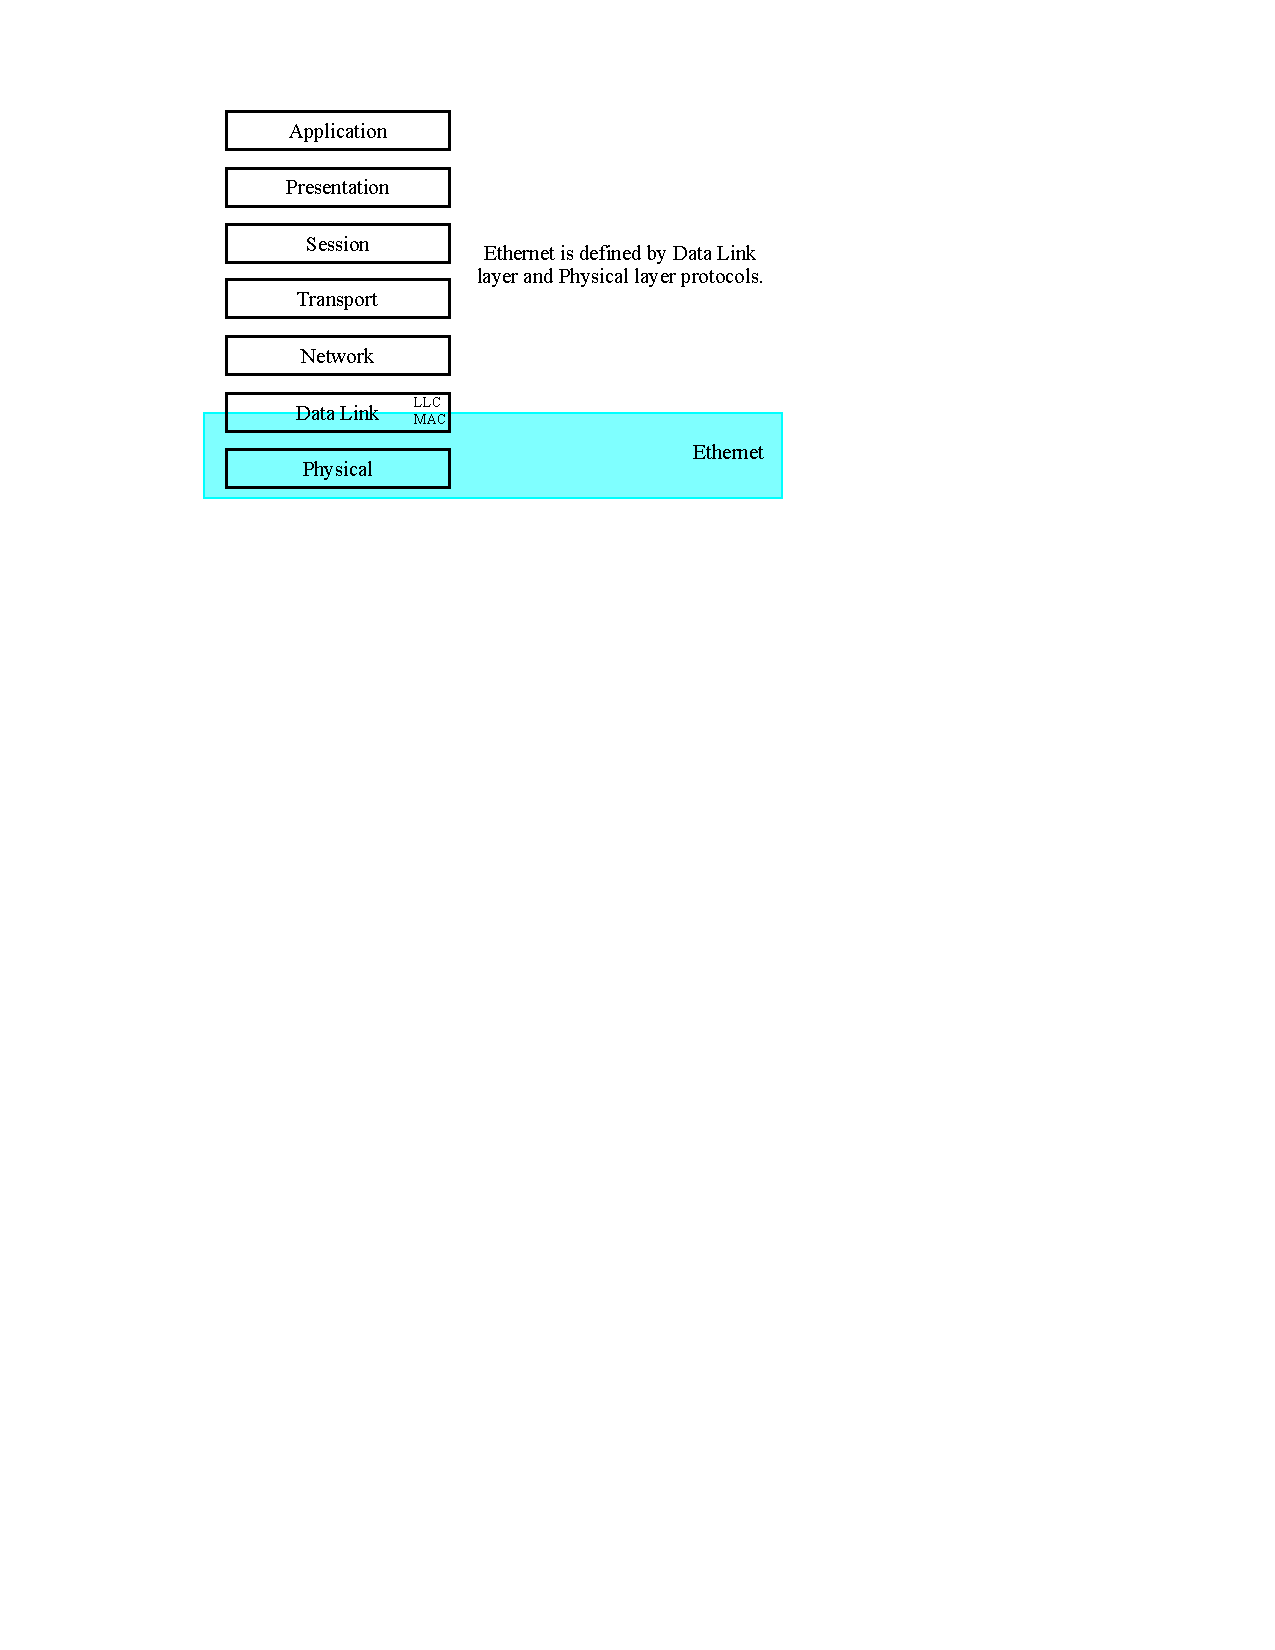
\includegraphics[scale=1]{figures/osi_ethernet_diagram.pdf}
	\caption{The block diagram that shows Ethernet standard inside the OSI model.} 
	\label{fig:osi_model}
\end{figure}

The DE2-115 board provides Ethernet support via the Marvell* 88E1111 Ethernet PHY chip, which is a physical layer device integrated with a 10/100/1000 Mbps Ethernet transceiver. To communicate with this chip, an Intel IP Core called Triple-Speed Ethernet can be used. This IP Core provides the features of a 10/100/1000-Mbps Ethernet Media Access Controller.

\section{Implementing a Triple-Speed Ethernet System}
This section describes how to implement the Triple-Speed Ethernet system shown in Figure~\ref{fig:bigsystem_block_diagram}. To start, create a new Quartus Prime project named {\it tse\_tutorial} in a new directory of the same name. Select the Cyclone\textsuperscript{\textregistered} IV E device {\sf EP4CE115F29C7}, which is the FPGA on the DE2-115 board.

\begin{figure}[H]
	\centering
	  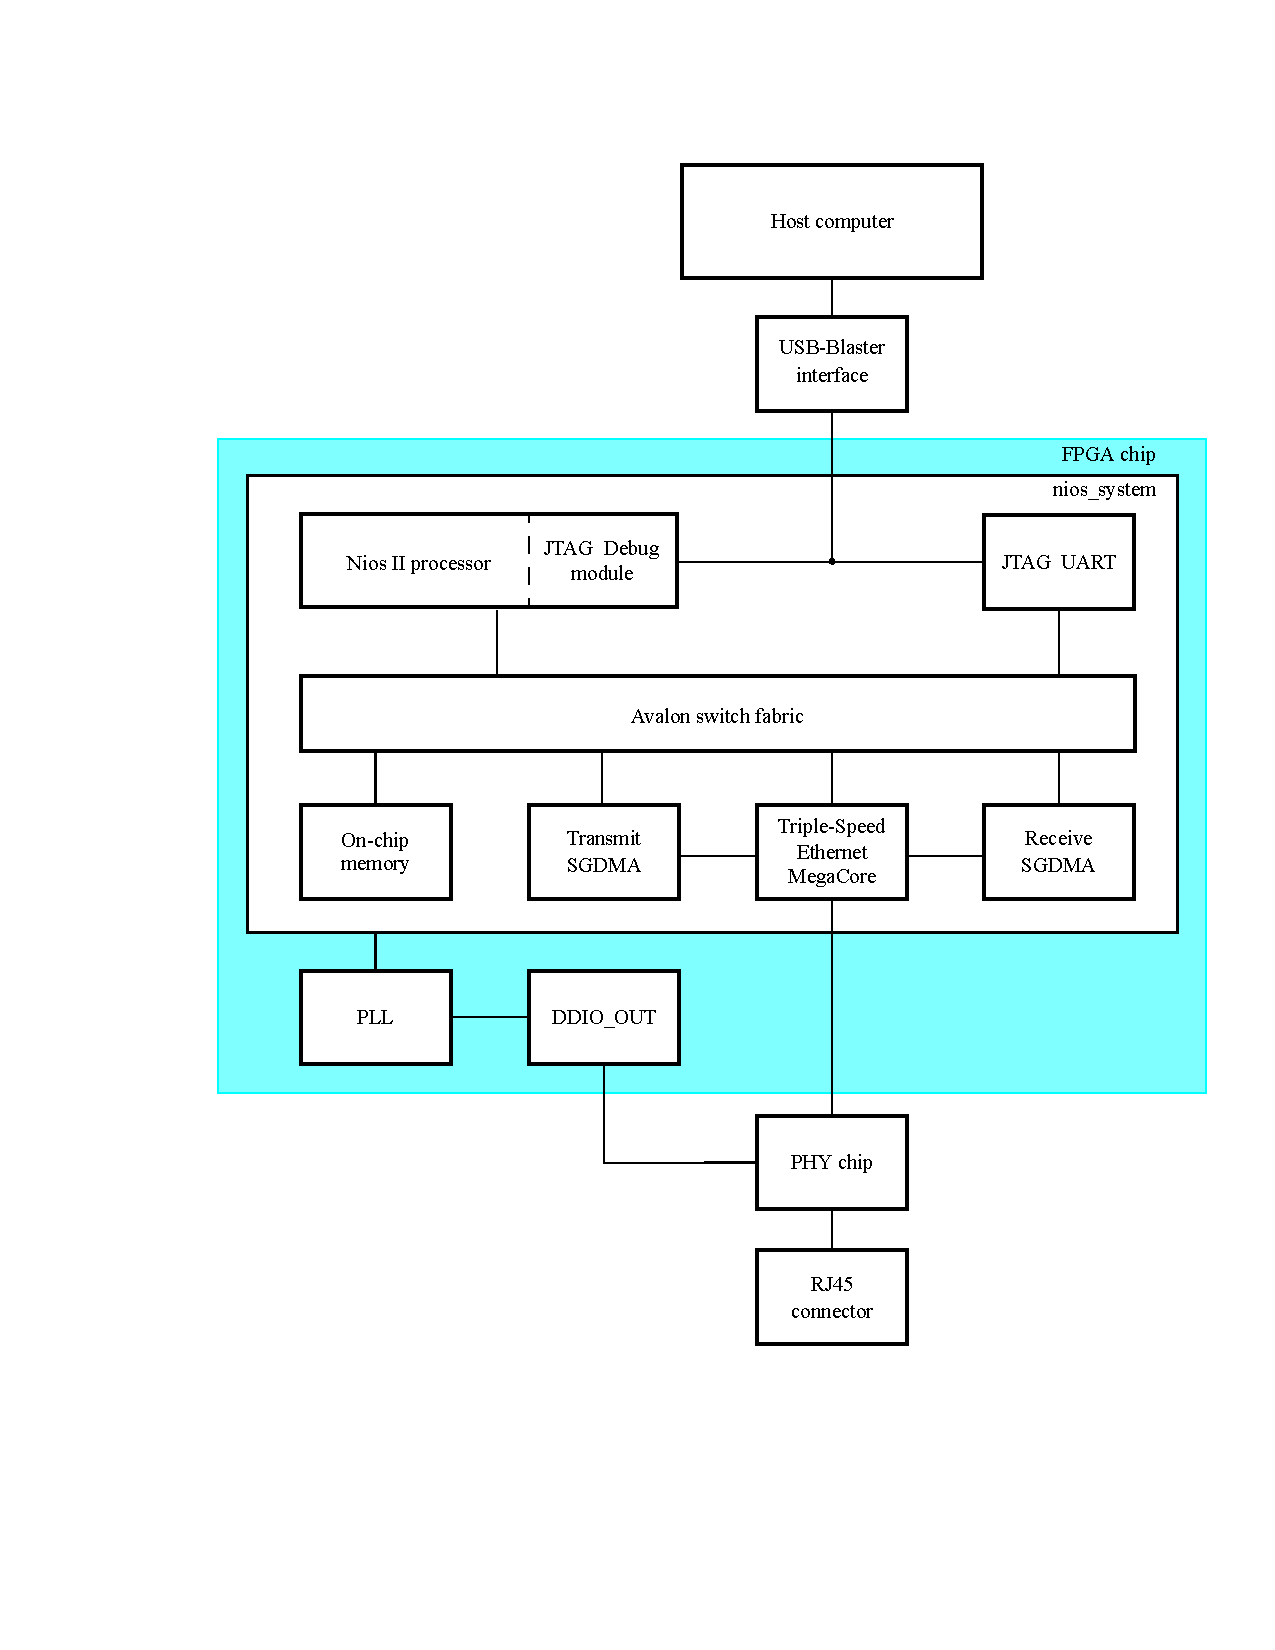
\includegraphics[scale=0.85]{figures/bigsystem_block_diagram.pdf}
	\caption{The block diagram of the Triple-Speed Ethernet system.} 
	\label{fig:bigsystem_block_diagram}
\end{figure}

\subsection{Creating the Nios\textsuperscript{\textregistered} System}
Most of the Triple-Speed Ethernet system can be built as a subsystem using the Platform Designer tool. The block diagram of this subsystem is shown in Figure~\ref{fig:subsystem_block_diagram}. 

\begin{figure}[H]
	\centering
	  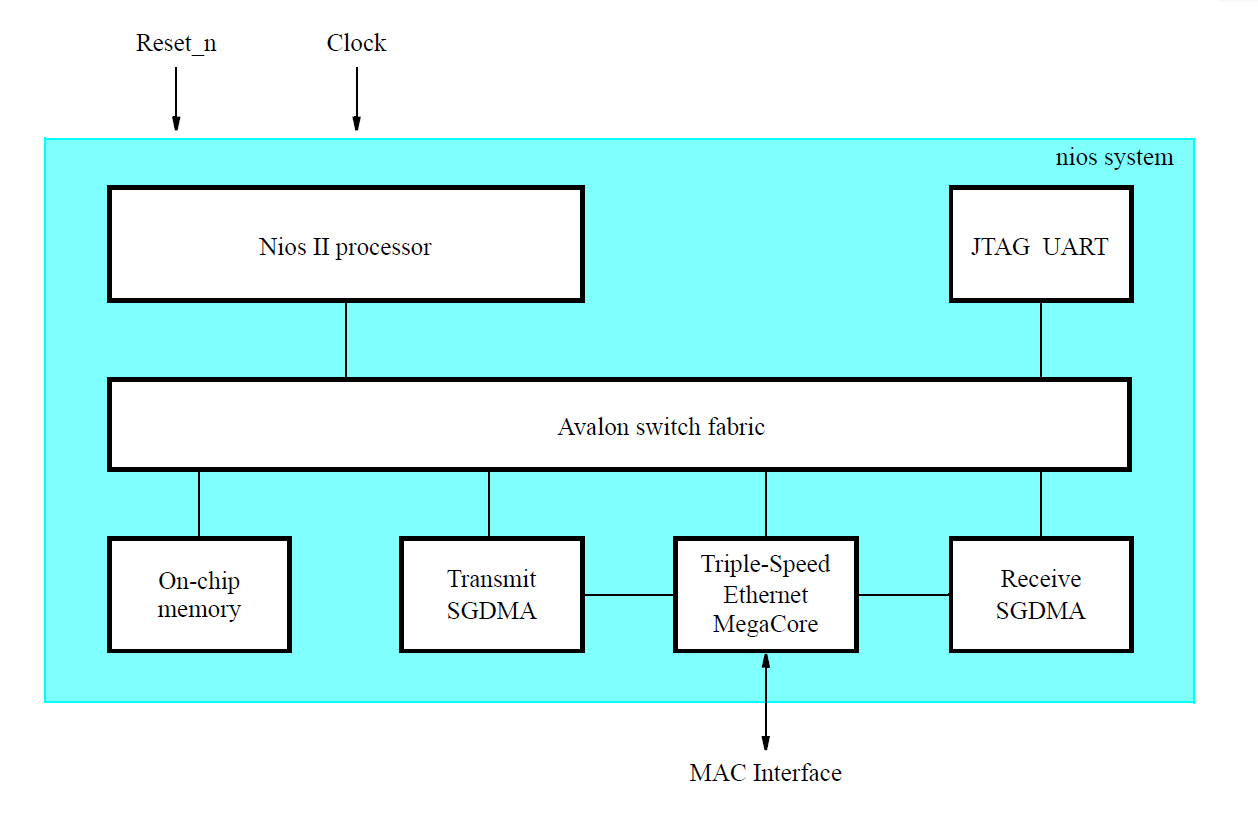
\includegraphics[scale=0.5]{figures/subsystem_block_diagram.png}
	\caption{The block diagram of the Platform Designer subsystem.} 
	\label{fig:subsystem_block_diagram}
\end{figure}

This subsystem takes a clock signal and an active-low reset signal as inputs, and communicates with the external PHY chip through a chosen interface. There is a Nios\textsuperscript{\textregistered} II processor to run application programs, a JTAG* UART component to support communication between the processor and the host computer, and a Triple-Speed Ethernet IP Core to implement the MAC sublayer and a partial Physical layer when needed based on the interface type. The two SGDMA controllers are used for the transmit and receive functions of the core. The on-chip memory is used for the program code, data, as well as descriptors for the SGDMA controllers. Note that the example system of this tutorial uses on-chip memory to simplify the system. For a larger system, it is better to use the SDRAM to have a larger memory for application programs.

To design the desired system, you should use the Platform Designer tool to add the components mentioned above and make necessary connections between them. You may want to rename the components as well to make the names more descriptive. Perform the following steps:

\begin{enumerate}
	\item Select {\bf Tools} > {\bf Platform Designer} to open the Platform Designer tool, and then save the file as {\it nios\_system.qsys}.

	\item Double-click on the clock source {\it clk\_}0 and change the {\bf Clock frequency} to 100000000 Hz (100MHz). Then, right-click on {\it clk\_}0 and rename it as {\it sys\_clk}. 

	\item Add a Nios II processor. The Nios II processor is used to run application programs that handle the data sent to or received from the Triple-Speed Ethernet IP Core. 
		\begin{itemize}	
			\item Select {\bf Processors and Peripherals} > {\bf Embedded Processors} > {\bf Nios II Processor} and click {\bf Add}.
			\item Choose {\bf Nios II/e}, which is the economy version of the processor. 
			\item Click {\bf Finish} to add the Nios II processor to the design, and rename it as {\it nios2}.
			\item Click on the {\bf Clock} column and select {\it sys\_clk} as the clock input to the processor, as shown in Figure~\ref{fig:processor_clk_select}. 
		\end{itemize}
		There may be some error messages at the bottom of the screen, because some parameters have not been specified yet. Ignore these messages as we will provide the necessary parameters later.

		\begin{figure}[H]
			\centering
			  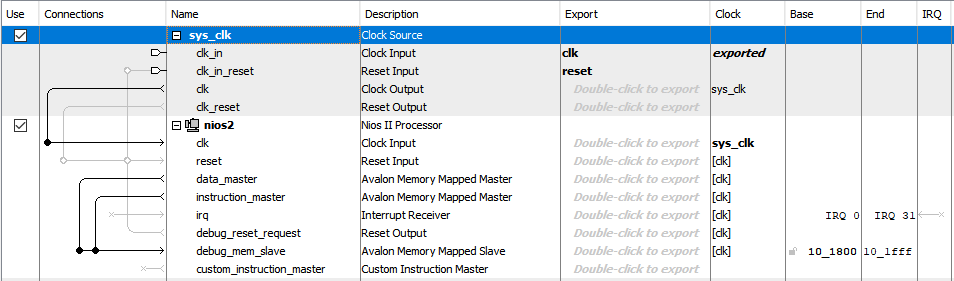
\includegraphics[scale=0.70]{figures/processor_clk_select.png}
			\caption{Select sys\_clk as the clock input of the processor.} 
			\label{fig:processor_clk_select}
		\end{figure}

	\item Add an on-chip memory, which will be used as the main memory to store programs and data for the processor. Any data received from the Triple-Speed Ethernet IP Core will be stored in this memory as well. 
		\begin{itemize}
			\item Select {\bf Basic Functions} > {\bf On Chip Memory} > {\bf On-chip Memory(RAM or ROM) Intel FPGA IP} and click {\bf Add}.
			\item Set the {\bf Total Memory Size} to 307200 bytes (300 KBytes), as shown in Figure~\ref{fig:onchip_memory1}. 
			\item Do not change the other default settings. 
			\item Click {\bf Finish} and rename the on-chip memory as {\it main\_memory}.
			\item Select {\it sys\_clk} as its clock input and connect its {\it s}1 slave port to both the {\it data\_master} and {\it instruction\_master} of the processor. 
		\end{itemize}
		
		\begin{figure}[H]
			\centering
			  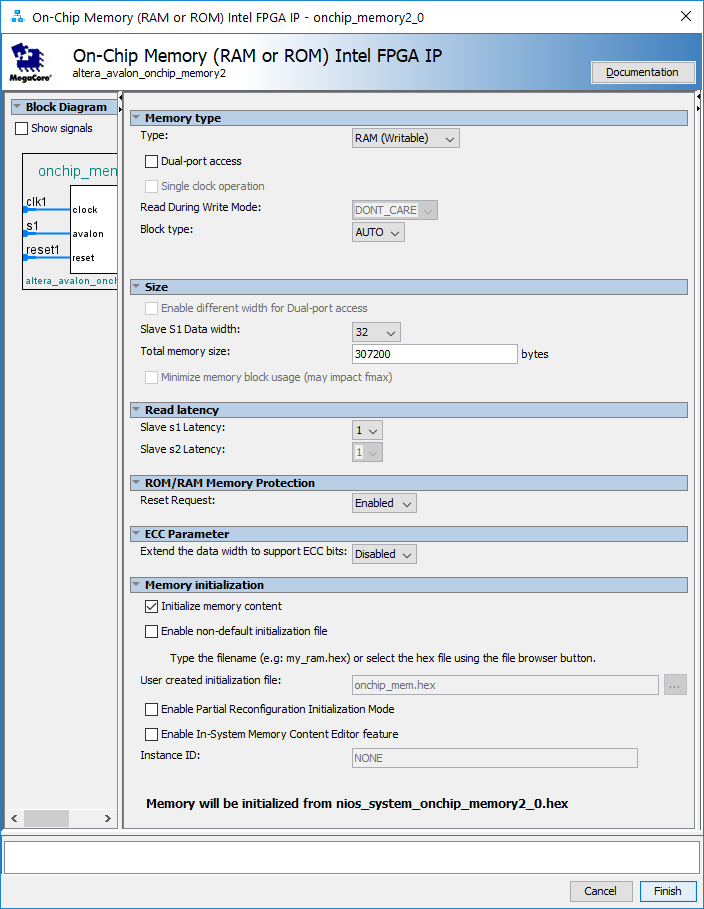
\includegraphics[scale=0.55]{figures/onchip_memory1.png}
			\caption{Settings for the on-chip memory.} 
			\label{fig:onchip_memory1}
		\end{figure}

	\item Add a JTAG UART component. With the JTAG UART component, the Nios II processor is able to send data to the host computer, such as information that needs to be printed out to the terminal in the application program.
		\begin{itemize}
			\item Select {\bf Interface Protocols} > {\bf Serial} > {\bf JTAG UART Intel FPGA IP} and click {\bf Add}.
			\item Do not change the default settings. 
			\item Click {\bf Finish} and rename it as {\it jtag\_uart}.
			\item Select {\it sys\_clk} as its clock input and connect its {\it avalon\_jtag\_slave} port to the {\it data\_master} port of the processor. 
			\item In the {\bf IRQ} column, connect the interrupt sender port from the {\it Interrupt Sender} slave port to the {\it interrupt receiver} port of the processor and set the IRQ number to be 0.
		\end{itemize}	
	
	\item Add a Triple-Speed Ethernet IP Core. It works as a Media Access Controller, which along with the Nios II processor and the external PHY chip are the key components of the Triple-Speed Ethernet system. For detailed information about this IP Core, refer to the {\it Triple-Speed Ethernet MegaCore Function User Guide}. 
		\begin{itemize}
			\item Select {\bf Interface Protocols} > {\bf Ethernet} > {\bf 1G Multi-rate Ethernet} > {\bf Triple-Speed Ethernet Intel FPGA IP}.
			\item Change the interface to be {\bf RGMII}, then select the {\bf MAC Options} tab.
			\item Select the following options: {\bf Enable MAC 10/100 half duplex support}, {\bf Include statistics counters}, {\bf Align packet headers to 32-bit boundary}, {\bf Enable magic packet detection}, and {\bf Include MDIO module (MDC/MDIO)}, as shown in Figure~\ref{fig:tse_ethernet_settings}. 
			\item Click {\bf Finish} and rename it as {\it tse}.
			\item Select {\it sys\_clk} as clock input for {\it receive\_clock\_connection}, {\it transmit\_clock\_connection} as well as {\it control\_port\_clock\_connection}. 
			\item Connect its {\it control\_port} slave port to the {\it data\_master} port of the processor.
			\item Export its {\it pcs\_mac\_tx\_clock\_connection}, {\it pcs\_mac\_rx\_clock\_connection}, {\it mac\_status\_connection}, 
			
			{\it mac\_rgmii\_connection}, and {\it mac\_mdio\_connection} by double-clicking on the {\bf Export} column.
		\end{itemize}
	
		\begin{figure}[H]
			\centering
			  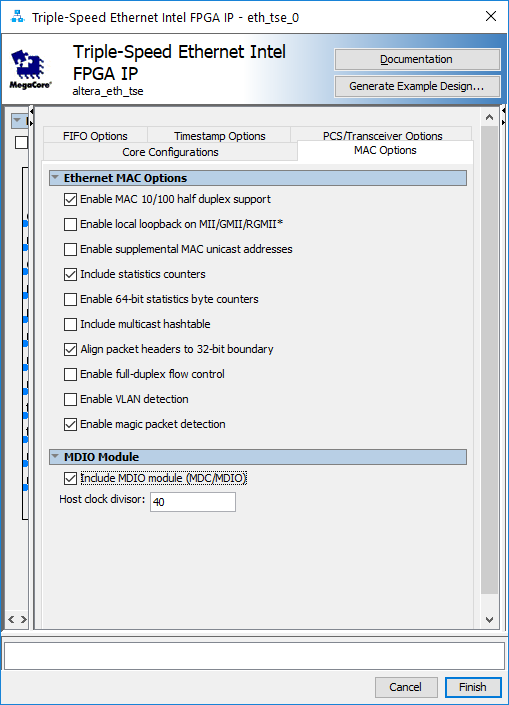
\includegraphics[scale=0.65]{figures/tse_ethernet_settings.png}
			\caption{Settings for the Triple-Speed Ethernet IP Core.} 
			\label{fig:tse_ethernet_settings}
		\end{figure}

	\item Add an SGDMA controller for receive operation. This controller will be set to transfer data from a streaming interface to a memory-mapped interface, so that data can be transferred from the Triple-Speed Ethernet IP Core to the on-chip memory. The controller will interrupt the processor whenever it finishes the data transfer. 
		\begin{itemize}
			\item Select {\bf Basic Functions} > {\bf DMA} > {\bf Scatter-Gather DMA Controller Intel FPGA IP}. 
			\item Select {\bf Stream To Memory} as the transfer mode and {\bf 6} as the sink error width, as shown in Figure~\ref{fig:sgdma_settings1}.  
			\item Click {\bf Finish} and rename it as {\it sgdma\_rx}.
			\item Select {\it sys\_clk} as its clock input and connect its {\it csr} slave port to the {\it data\_master} port of the processor.
			\item Connect its {\it m\_write} master port to the {\it s}1 port of the {\bf main\_memory} and its {\it in} streaming sink to the {\it receive} streaming source of the {\bf tse} component.		
			\item In the {\bf IRQ} column, connect the interrupt sender port from the {\it csr} slave port to the interrupt receiver port of the processor and set the IRQ number to be 1.
		\end{itemize}
		
		\begin{figure}[H]
			\centering
			  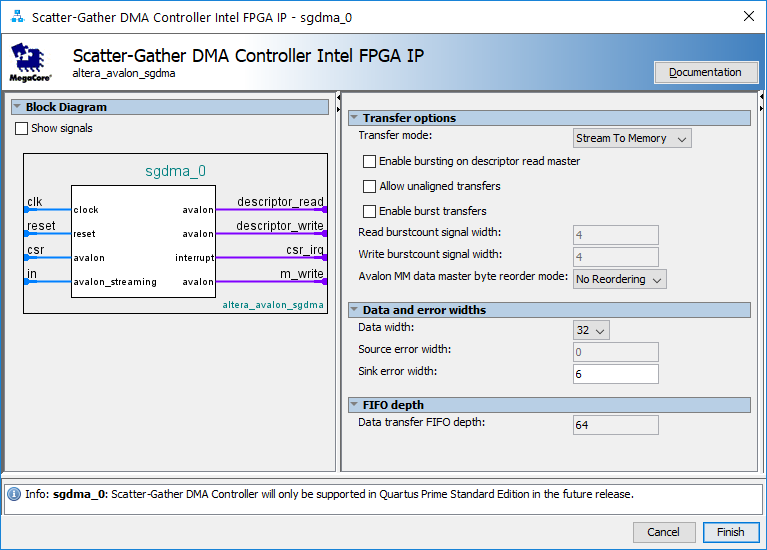
\includegraphics[scale=0.65]{figures/sgdma_settings1.png}
			\caption{Settings for the SGDMA controller.} 
			\label{fig:sgdma_settings1}
		\end{figure}		
	
	\item Add another SGDMA controller for transmit operation. This controller governs the reading of data from the on-chip memory {\it main\_memory} and sending it to the Triple-Speed Ethernet IP Core. 
		\begin{itemize}
			\item Select {\bf Basic Functions} > {\bf DMA} > {\bf Scatter-Gather DMA Controller Intel FPGA IP}. 
			\item As depicted in Figure~\ref{fig:sgdma_settings2}, select {\bf Memory To Stream} as the transfer mode and {\bf 1} as the source error width. 
			\item Click {\bf Finish} and rename it as {\it sgdma\_tx}.
			\item Select {\it sys\_clk} as its clock input and connect its {\it csr} slave port to the {\it data\_master} port of the processor.
			\item Connect its {\it m\_read} master port to the {\it s}1 port of the {\bf main\_memory} and its {\it out} streaming source to the {\it transmit} streaming sink of the {\bf tse} component. 
			\item In the {\bf IRQ} column, connect its interrupt sender to the interrupt receiver of the processor and set the IRQ number to be 2. 
		\end{itemize}

		\begin{figure}[H]
			\centering
			  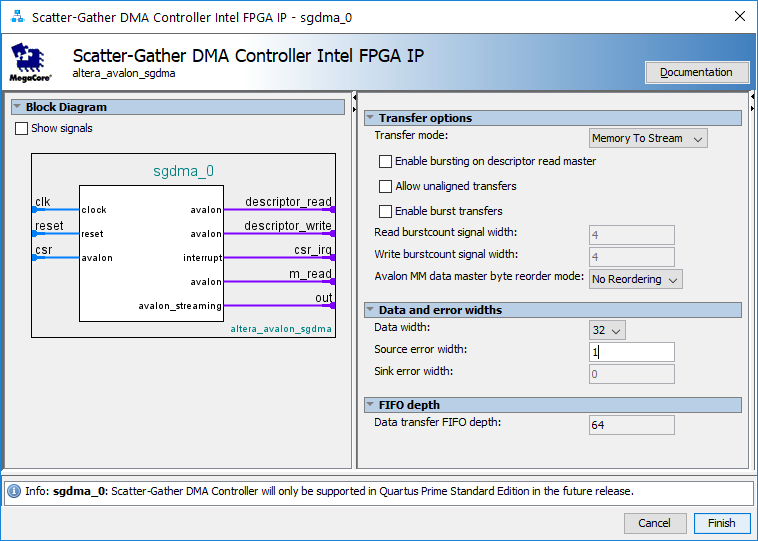
\includegraphics[scale=0.65]{figures/sgdma_settings2.png}
			\caption{Settings for the other SGDMA controller.} 
			\label{fig:sgdma_settings2}
		\end{figure}
	
	\item Add another on-chip memory. Unlike the {\it main\_memory} part, this on-chip memory is used to store only the descriptors of the SGDMA controllers.
		\begin{itemize}
			\item Select {\bf Basic Functions} > {\bf On Chip Memory} > {\bf On-chip Memory(RAM or ROM) Intel FPGA IP} and click {\bf Add}.
			\item Leave the default settings and click {\bf Finish}. 
			\item Rename it as {\it descriptor\_memory} and select {\it sys\_clk} as its clock input
			\item Connect its {\it s}1 slave port to the {\it data\_master} of the processor, the {\it descriptor\_read} and the {\it descriptor\_write} ports for both {\bf sgdma\_tx} and {\bf sgdma\_rx}. This will guarantee that this on-chip memory is accessible for the processor and the two SGDMA controllers. 
		\end{itemize}
	
	\item Now, all the components have been added, but the system is not complete as there are several error messages displayed. 
		\begin{itemize}
			\item Click on the drop-down menu {\bf System} and click {\bf Assign Base Address} to auto assign base addresses for all the components.
			\item Under the same menu, click {\bf Create Global Reset Network} to connect the reset signals to form a global reset network.
			\item Double-click the Nios II processor {\it nios2} to edit its settings.  Change both the reset and exception vector memory options to {\bf main\_memory.s1}, as shown in Figure~\ref{fig:nios2_settings}. Then click {\bf Finish}. The final system is shown in Figure ~\ref{fig:nios2_system}.
		\end{itemize}

		\begin{figure}[H]
			\centering
			  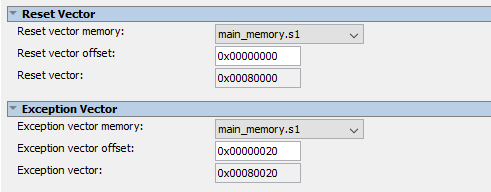
\includegraphics[scale=0.55]{figures/nios2_settings.png}
			\caption{Settings for the Nios II processor.} 
			\label{fig:nios2_settings}
		\end{figure}
	
		\begin{figure}[H]
			\centering
			  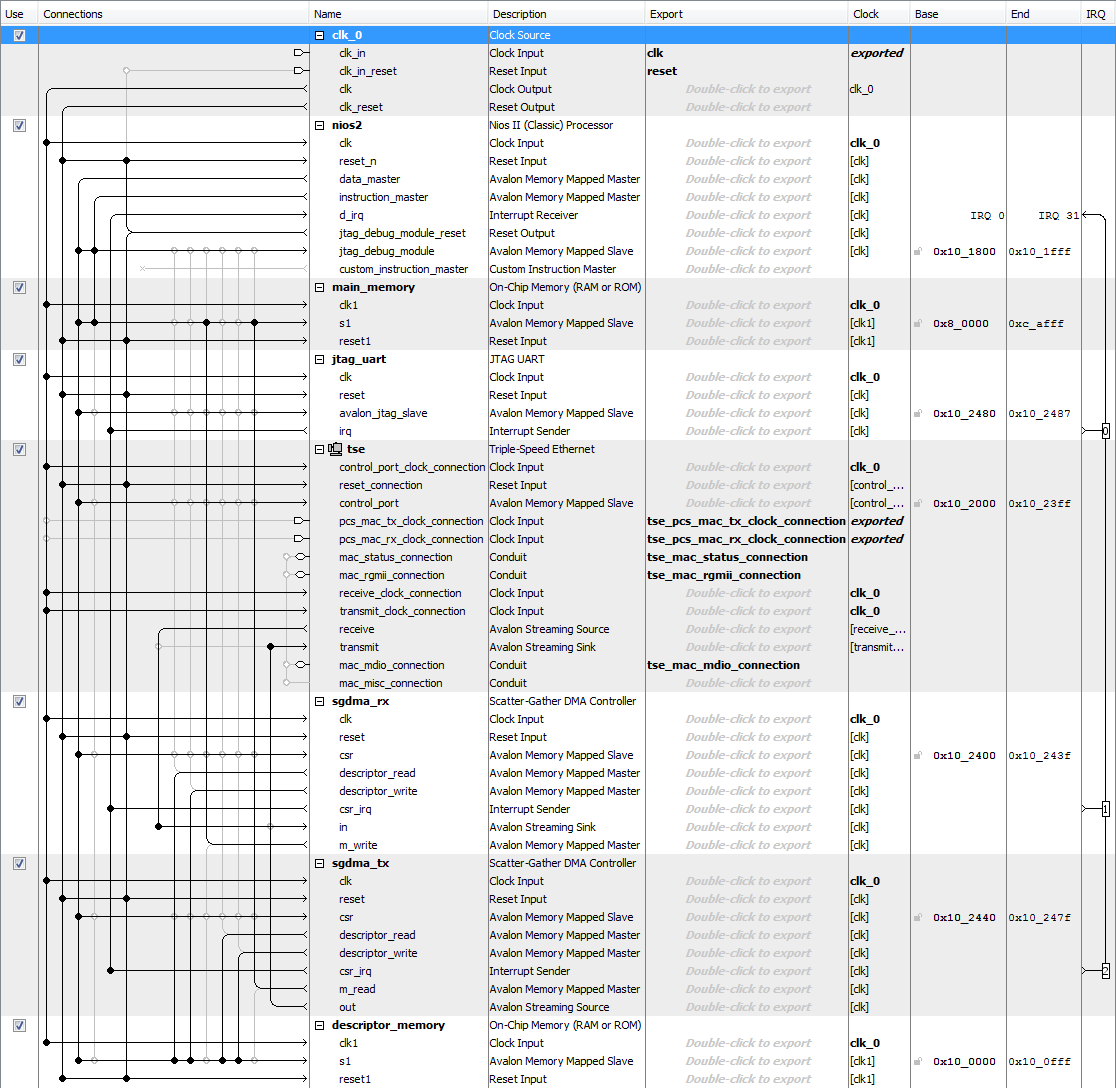
\includegraphics[scale=0.55]{figures/nios2_system.png}
			\caption{Nios II system with connections.} 
			\label{fig:nios2_system}
		\end{figure}	
	
	\item After you have resolved all error messages, you can generate the system. 
		\begin{itemize}
			\item Select {\bf Generate > Generate HDL...}.
			\item Uncheck the {\bf Create block symbol file (.bsf)} in the {\bf Synthesis} section as shown in Figure~\ref{fig:qsys_generation}.
			\item Click {\bf Generate} on the bottom of the window.
			\item When successfully completed, the generation process produces the message ``Generate Completed''.
		\end{itemize}
	
		\begin{figure}[H]
			\centering
			  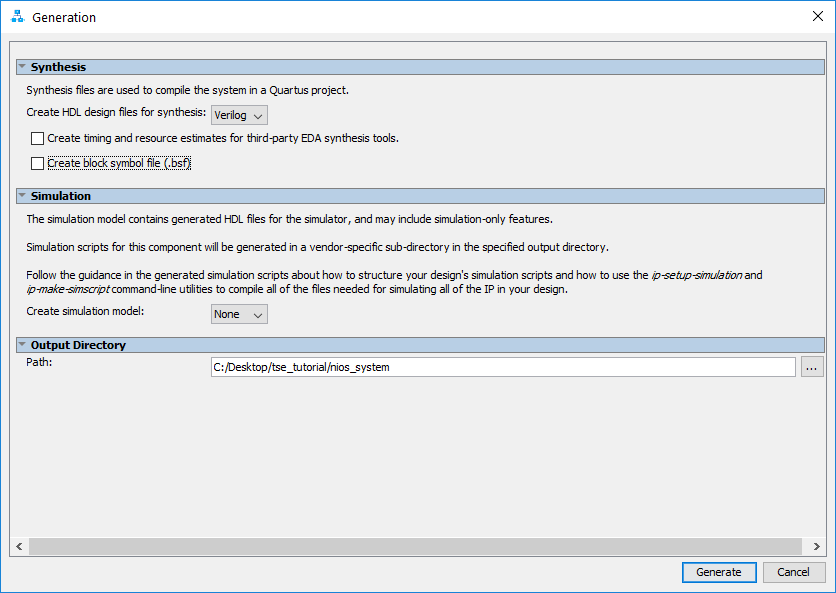
\includegraphics[scale=0.55]{figures/qsys_generation.png}
			\caption{Settings for Generating Platform Designer.} 
			\label{fig:qsys_generation}
		\end{figure}	
\end{enumerate}

After the generation is completed, you can have a look at the example of how to instantiate the system you built by selecting {\bf Generate > Show Instantiation Template} as shown in Figure~\ref{fig:hdl_example}. Later you will use this template to instantiate this subsystem in your top-level module. 

		\begin{figure}[H]
			\centering
			  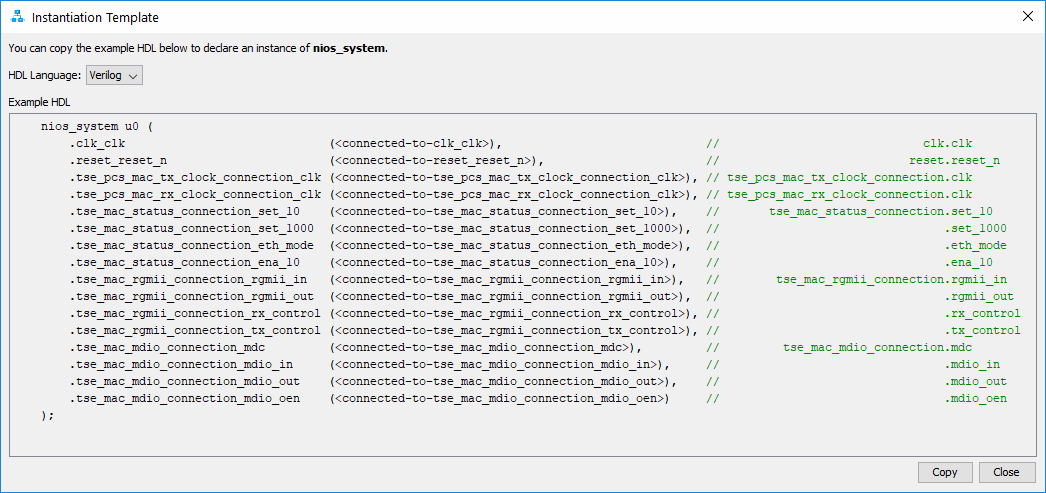
\includegraphics[scale=0.5]{figures/hdl_example.png}
			\caption{HDL example for the Platform Designer subsystem.} 
			\label{fig:hdl_example}
		\end{figure}

\subsection{Adding Additional Modules}
Besides the subsystem built using Platform Designer, you need a Phase-Locked Loop (PLL) module to generate clocks with different frequencies to make the Triple-Speed Ethernet system work properly. The PLL will take a 50 MHz input clock, and output the desired clocks. To add the PLL block, perform the following:

\begin{enumerate}
	\item Select {\bf Tools} > {\bf IP Catalog} from the main Quartus window. %Select {\bf Create a new custom megafunction variation} when the window appears, and then click {\bf Next}.
	\item In the pop-up panel, select {\bf Library > Basic Functions > Clocks; PLLs and Resets > PLL > ALTPLL} and click {\bf Add...} button.
	%\item Expand the {\bf I/O} directory under {\bf Installed Plug-Ins} by clicking the + icon left of the directory name, and click {\bf ALTPLL}.
	\item Choose the {\bf Verilog} as the output file type for your design, and specify {\it my\_pll.v} as the name of the output file as shown in Figure~\ref{fig:pll_settings1}, and click {\bf OK}.
	
	\begin{figure}[H]
		\centering
		  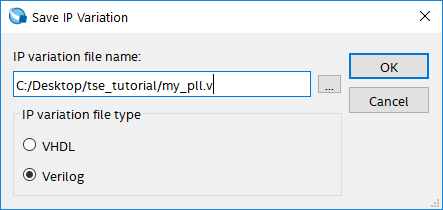
\includegraphics[scale=0.65]{figures/pll_settings1.png}
		\caption{The IP Catalog.} 
		\label{fig:pll_settings1}
	\end{figure}

	\item Under the {\bf Parameter Settings} tab, set {\bf What is the frequency of the inclk0 input?} to 50 MHz as shown in Figure~\ref{fig:pll_settings2}.
	
	\begin{figure}[H]
		\centering
		  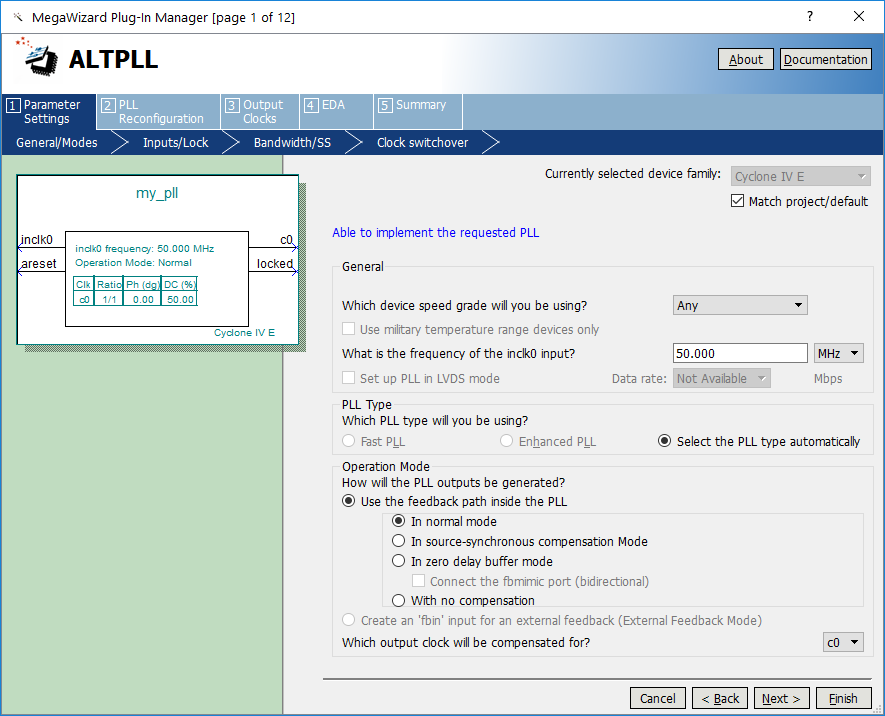
\includegraphics[scale=0.6]{figures/pll_settings2.png}
		\caption{Settings for General/Mode section.} 
		\label{fig:pll_settings2}
	\end{figure}
	
	\item Under the {\bf Output Clocks} tab, enter 100 MHz after selecting {\bf Enter output clock frequency} as shown in Figure~\ref{fig:pll_settings3}. This will cause the PLL to output a 100-MHz clock for the system clock {\it sys\_clk} . Click {\bf Next} to go to the {\bf clk\_c1} section.
	
	\begin{figure}[H]
		\centering
		  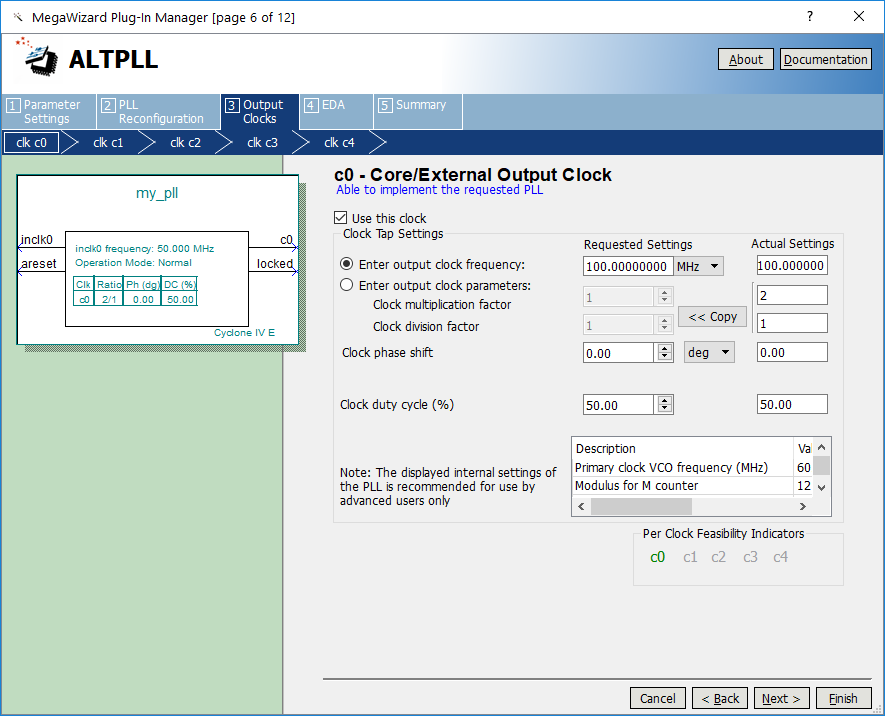
\includegraphics[scale=0.5]{figures/pll_settings3.png}
		\caption{Settings for output c0.} 
		\label{fig:pll_settings3}
	\end{figure}
	
	\item Select the checkbox {\bf Use this clock} and set the output clock frequency to 125 MHz using the same procedure as in the last step. This 125-MHz clock will serve as the transmission clock for the Triple-Speed Ethernet IP Core when operating in the Gigabit mode.
	\item Repeat the same procedure to create a clock with 25 MHz and one with 2.5 MHz. These clocks will be used when the IP Core operates in 100 Mbps mode and 10 Mbps mode respectively. 
	\item Under the {\bf Summary} tab, uncheck {\bf my\_pll\_bb.v} as shown in Figure~\ref{fig:pll_settings4}, and then click {\bf Finish} to generate the files.	
	
	\begin{figure}[H]
		\centering
		  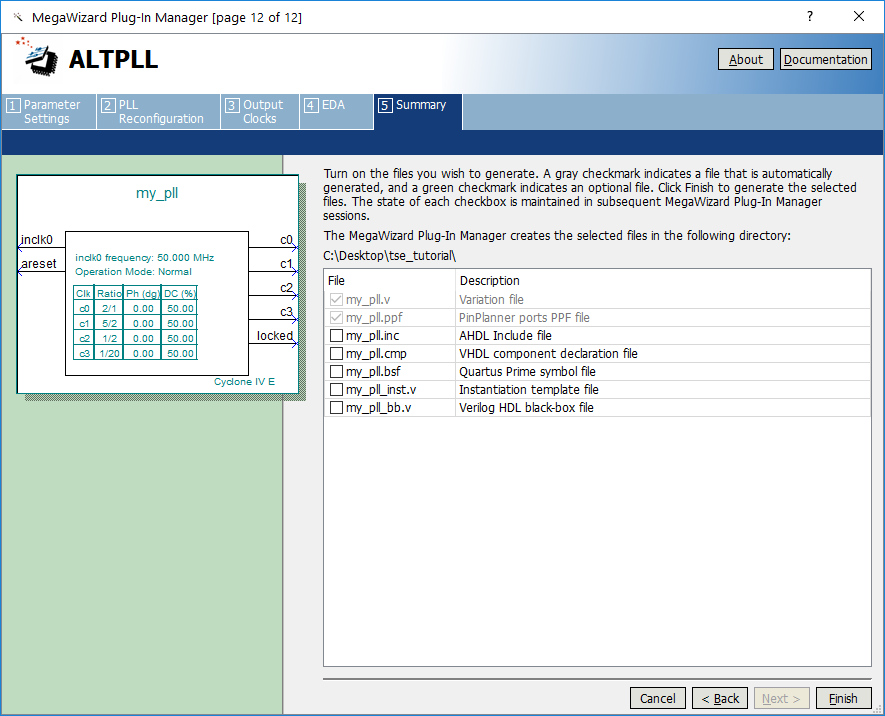
\includegraphics[scale=0.6]{figures/pll_settings4.png}
		\caption{Settings for Summary tab.} 
		\label{fig:pll_settings4}
	\end{figure}
	
	\item If a pop-up box appears, click {\bf Yes} to include the generated IP file in the project.
\end{enumerate}

Another module needed is a DDIO\_OUT register. By using the DDIO\_OUT register for the transmission clock, outputting to the external PHY chip will create a very accurate edge-aligned clock-data relationship. Thus, we can maximize the timing margin on the data capture to improve the performance of the system.

\begin{enumerate}
	\item Open the IP Catalog to create a new custom IP Core variation.
	\item Select {\bf Basic Functions > I/O > ALTDDIO\_OUT} and enter {\it my\_ddio\_out.v} as the file name. Click {\bf Next}.
	\item In the window in Figure~\ref{fig:ddio_settings}, set the {\bf width} to {\bf 1} bit.  Also select {\bf Not used} for the {\bf asynchronous clear and asynchronous set ports} options.

	\begin{figure}[H]
		\centering
		  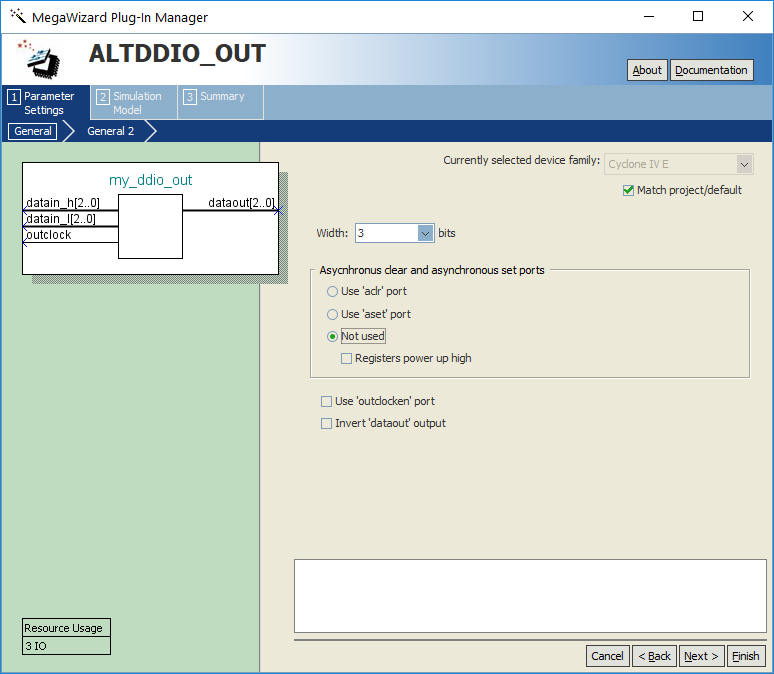
\includegraphics[scale=0.6]{figures/ddio_settings.png}
		\caption{Settings for the DDIO\_OUT register.} 
		\label{fig:ddio_settings}
	\end{figure}

	\item Navigate to the {\bf Summary} tab and uncheck all the uncheckable files as shown in Figure~\ref{fig:ddio_settings2}. Then click {\bf Finish}.
\end{enumerate}

	\begin{figure}[H]
		\centering
		  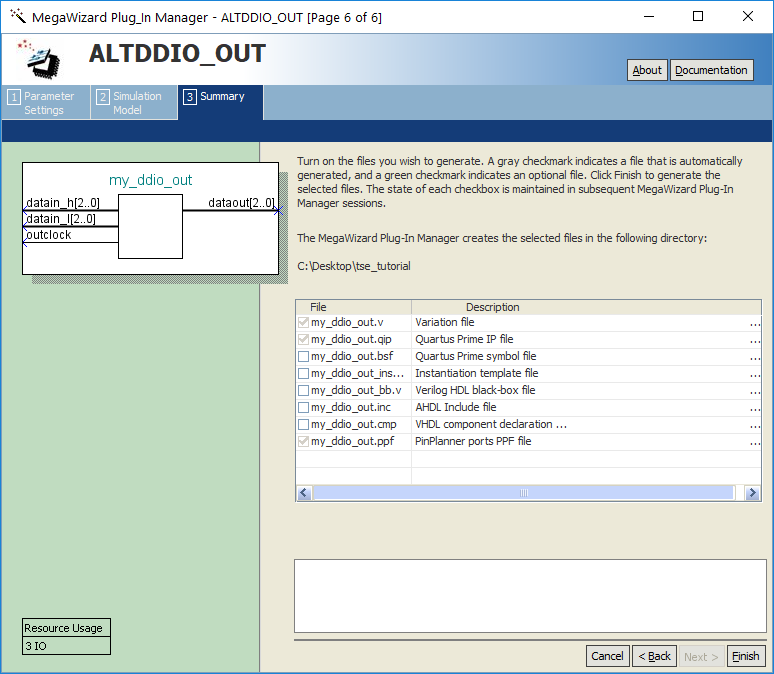
\includegraphics[scale=0.6]{figures/ddio_settings2.png}
		\caption{Settings for the Summary tab of DDIO\_OUT register.} 
		\label{fig:ddio_settings2}
	\end{figure}

\subsection{Integrating Modules into the Quartus\textsuperscript{\textregistered} Prime Project}
Next, you have to instantiate the nios\_system and the two additional modules within the top-level module. The complete Verilog file for top-level module is provided in the design\_files folder along with this tutorial. You may notice that the signals from {\it tse\_mac\_conduit} are connected to the pins related to Ethernet1, but the MDIO signals are connected to Ethernet0 as well. This is because an extra Ethernet port is required to implement a loopback functionality to mimic the actual communication between ports for the demonstration application in the next section. 

To complete the hardware design, perform the following:

\begin{enumerate}
	\item Copy the provided Verilog file {\it tse\_tutorial.v} and the timing constraint file {\it tse\_tutorial.sdc} to project directory. The timing constraint file is required by the TimeQuest Tool to properly evaluate the timing of your system.
	\item Select {\bf Assignments} > {\bf Settings...} to add the {\it tse\_tutorial.v}, {\it tse\_tutorial.sdc} and {\it nios\_system.qip} files to the Quartus Prime project. Along with the {\it .qip} files for the two modules generated by the IP Catalog before, all the files included in the project are shown in Figure~\ref{fig:files_settings}. 
	
	\begin{figure}[H]
		\centering
		  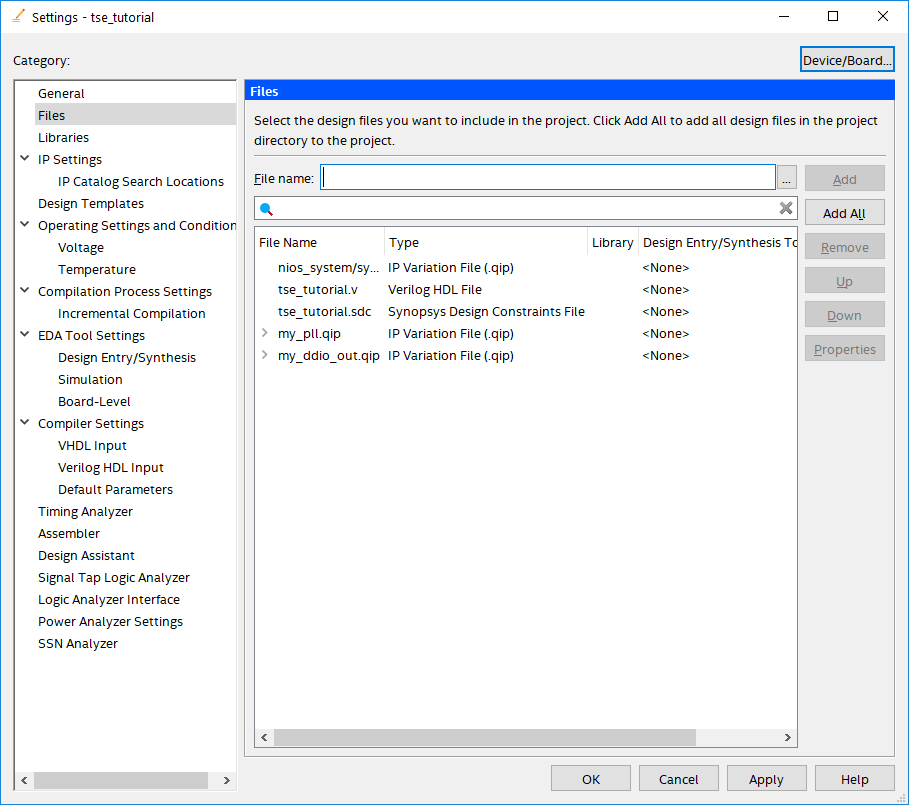
\includegraphics[scale=0.6]{figures/files_settings.png}
		\caption{Settings for Files included in the Project.} 
		\label{fig:files_settings}
	\end{figure}
			
	\item Select {\bf Assignments} > {\bf Import Assignments...} to add the necessary pin assignments for the DE2-115 board to your project. The pin assignment file {\it DE2\_115\_pin\_assignments.qsf} can be found in the design\_files folder.
	\item Select {\bf Processing} > {\bf Start Compilation} to compile your project in Quartus Prime software. 
\end{enumerate}


\section{Application Program for the Ethernet System}
After building the hardware system, you can now download the circuit onto the FPGA and run an application program. A demonstration application is provided with this tutorial. The program will print what the user types in the terminal window and send the message through the Ethernet port when the user presses the {\bf Enter} key. If at any time a message is received, the received message will be printed in the terminal window. 

\subsection{A C-Language Demonstration Program}
The C-language source file {\it tse\_tutorial.c} is given in the design\_files folder. To help you understand the source code, some sections of the code are explained below.

At the beginning of the source code, some necessary variables are declared as global variables. As shown in Figure~\ref{fig:allocate_packets}, this section of the code allocates memory to store both the transmission and received frames. Also, it performs the necessary initialization for the transmission frames. The all 1's destination address means that this frame is a broadcast frame, while the source address indicates the MAC address of the source hardware device. The length of the payload data is a fixed value of 46 characters indicated by the 0x2E under the length section. A termination character `$\backslash$0' is used to determine the actual end of the message sent. 

\begin{figure}[H]
	\begin{lstlisting}[language=C]
unsigned char tx_frame[1024] = {
    0x00,0x00,                     // for 32-bit alignment
    0xFF,0xFF,0xFF,0xFF,0xFF,0xFF, // destination address (broadcast)
    0x01,0x60,0x6E,0x11,0x02,0x0F, // source address
    0x00,0x2E,                     // length or type of the payload data
    '\0'                           // payload data (ended with termination char)
};

unsigned char rx_frame[1024] = { 0 };
	\end{lstlisting}
	\caption{Allocating memory for transmission and received frames.}
	\label{fig:allocate_packets}
\end{figure}

Pay attention to the keyword {\bf \_\_attribute\_\_} shown in Figure~\ref{fig:attribute_keyword}. By adding {\bf \_\_attribute\_\_ (( section ( ``.descriptor\_memory'' )))} to the end of the declaration, you tell the compiler to place certain variables into the ``.descriptor\_memory'' section. This matches the requirement of the previous Ethernet system that the descriptors for the SGDMA controllers should be put in the memory called {\it descriptor\_memory}. Variables without this keyword will be placed along with the program code into the other memory called the {\it main\_memory}. 

\begin{figure}[H]
	\begin{lstlisting}[language=C]
alt_sgdma_descriptor tx_descriptor __attribute__ ((section(".descriptor_memory")));
alt_sgdma_descriptor tx_descriptor_end __attribute__ ((section(".descriptor_memory")));

alt_sgdma_descriptor rx_descriptor __attribute__ ((section(".descriptor_memory")));
alt_sgdma_descriptor rx_descriptor_end __attribute__ ((section(".descriptor_memory")));
	\end{lstlisting}
	\caption{Allocating memory for descriptors in the ``descriptor\_memory''.}
	\label{fig:attribute_keyword}
\end{figure}

In the {\bf main} function, the initialization of the SGDMA controllers is performed first. This involves opening the SGDMA devices, setting up the interrupt routine, creating a descriptor, and setting up transfers for the descriptor. This is done by using the Application Programming Interface (API) for the SGDMA controller. For more details about how to use these API functions, refer to the chapter {\it Scatter-Gather DMA Controller Core} in {\it Embedded Peripherals IP User Guide}.

The next piece of code is the process of initializing the Triple-Speed Ethernet IP Core and the external PHY chips. This code is shown in Figure~\ref{fig:tse_initialization}. It is performing the following:
\begin{enumerate}
	\item Define a pointer to the base address of the Triple-Speed Ethernet IP Core.
	\item Give the Triple-Speed Ethernet IP Core its MAC address (0x0F02116E6001), which matches the source address of the transmission frame. 
	\item Write the PHY addresses to the IP Core for access to the specific external PHY chips using MDIO interface. 
	\item Write to register 20 of the first PHY chip, which is the PHY chip for the Ethernet 0 port, to set up the line loopback functionality. This will enable the Ethernet 0 port to send back all the frames it received.
	\item Write to register 16 of the second PHY chip to enable automatic crossover for all modes. With this option turned on, you can use any Ethernet cable to connect the Ethernet ports rather than using a cross-over cable only.
	\item Write to register 20 of the second PHY chip to set up the phase-shift delay for the input and output clocks. This is important because the Gigabit Ethernet is working at the double data rate. By shifting the input and output clocks, the clock edges will be aligned with the center of the data to ensure correct data capturing. 
	\item After turning the phase-shift delay option on, you need to software reset the PHY chip and then wait for the reset bit to be cleared. 
	\item Finally, enable read and write transfers, Gigabit Ethernet operation, and CRC forwarding. You can write different values into this register to tell the IP Core to operate at 100 Mbps or 10 Mbps mode. For example, you can write 0x00000043 for operating at 100 Mbps and write 0x02000043 for 10 Mbps. More details can be found in {\it Triple-Speed Ethernet IP Core Function User Guide}. 
\end{enumerate}

\begin{figure}[H]
	\begin{lstlisting}[language=C]
// Triple-speed Ethernet IP Core base address
volatile int *tse =(int *) 0x00102000;

// Initialize the MAC address
*(tse + 3) = 0x116E6001;
*(tse + 4) = 0x00000F02;

// Specify the addresses of the PHY devices to be accessed through MDIO interface
*(tse + 0x0F) = 0x10;
*tse + 0x10 = 0x11;

// Write to register 20 of the PHY chip for Ethernet port 0 to set up line loopback
*(tse + 0x94) = 0x4000;

// Write to register 16 of the PHY chip for Ethernet port 1 to enable automatic crossover for all modes
*(tse + 0xB0) = *(tse + 0xB0) | 0x0060;

// Write to register 20 of the PHY chip for Ethernet port 2 to set up delay for input/output clk
*(tse + 0xB4) = *(tse + 0xB4) | 0x0082;

// Software reset the second PHY chip and wait
*(tse + 0xA0) = *(tse + 0xA0) | 0x8000;
while (*(tse + 0xA0) & 0x8000)
    ;

// Enable read and write transfers, gigabit Ethernet operation, and CRC forwarding
*(tse + 2) = *(tse + 2) | 0x0000004B;
	\end{lstlisting}
	\caption{Initialization Process for Triple-Speed Ethernet and external PHY chips}
	\label{fig:tse_initialization}
\end{figure}

After you enable the read and write transfers, the Triple-Speed Ethernet IP Core will start working. Then the main loop is entered which sends data typed by the user and prints messages that are received. The last part of the code is the interrupt routine. Whenever an interrupt is raised, the interrupt routine will be executed to:

\begin{itemize}
	\item Erase the user's current message from the screen.
	\item Print the received message.
	\item Reprint the user's message that was erased.
\end{itemize}

\subsection{Running the Application Program}
In this section we will use the {\it \productNameMed{}}, provided by the Intel FPGA University Program for use with the DE-series boards. The Monitor Program provides a simple means for compiling, assembling and downloading of programs onto a DE-series board. It also makes it easy for the user to perform debugging tasks. A description of this software is available in the {\it \productNameMed{}} tutorial. 

To run the demonstration application program above, perform the following steps:

\begin{enumerate}
	\item Connect the DE2-115 board to the host computer and make sure it is powered on.
	
	\item Create a new subdirectory named {\it app\_software} within the {\it tse\_tutorial} project directory. Copy the provided file {\it tse\_tutorial.c} into this new directory. 
	
	\item Open the Monitor Program and create a project named {\it tse\_tutorial} in the above directory.
	
	\item Select {\bf Nios II} as the architecture. Click {\bf Next}. 
	
	\item In the window in Figure~\ref{fig:monitor_figure1}, select {\bf Custom System} as the system type and browse to find the appropriate {\it .sopcinfo} and {\it .sof} files. Select {\bf Not Required} for the preloader. Click {\bf Next}.
	
	\begin{figure}[H]
		\centering
		  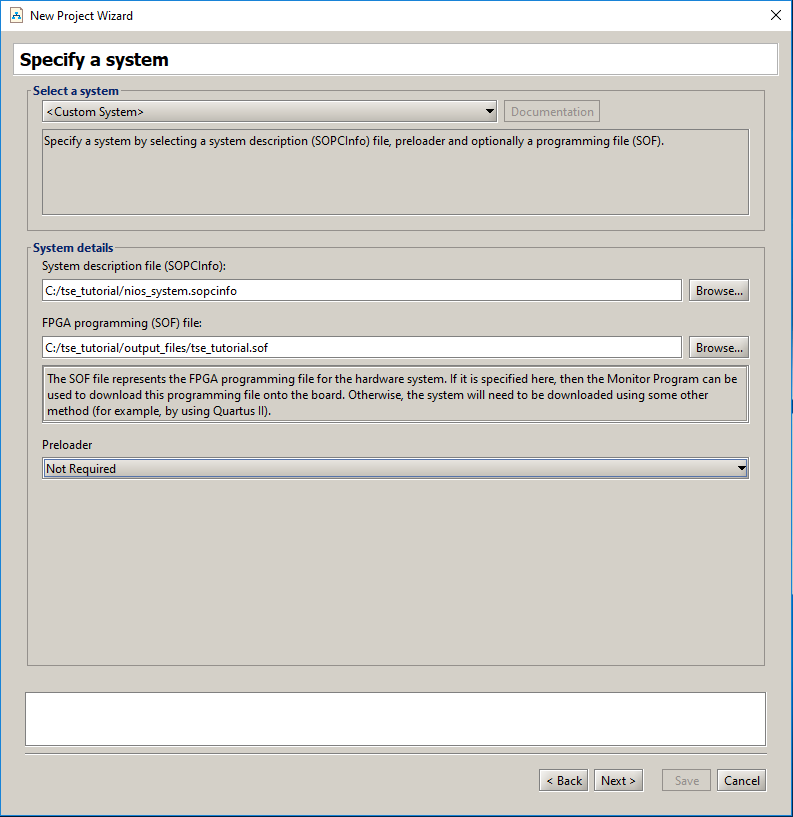
\includegraphics[scale=0.55]{figures/monitor_figure1.png}
		\caption{Specifying a system.} 
		\label{fig:monitor_figure1}
	\end{figure}	
	
	\item In the next window select {\bf Program with Device Driver Support} as the program type. Click {\bf Next}.
	
	\item Then add the {\it tse\_tutorial.c} file and click {\bf Next}.
	
	\item In the window in Figure~\ref{fig:monitor_figure2}, if the physical connection exists between the host computer and your DE2-115 board you should see {\bf USB-Blaster [USB-0]} under the {Host Connection} drop-down list. Otherwise, you should check the connection and make sure that the USB-Blaster driver is correctly installed. Then click {\bf Save}.

	\begin{figure}[H]
		\centering
		  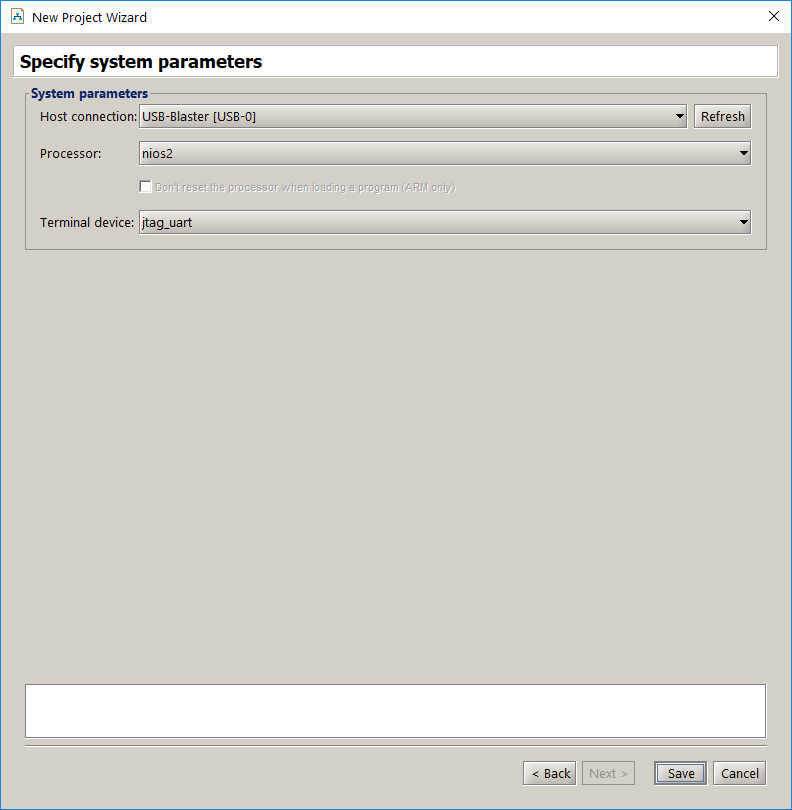
\includegraphics[scale=0.7]{figures/monitor_figure2.png}
		\caption{Check physical connection between the host computer and the DE2-115 board.} 
		\label{fig:monitor_figure2}
	\end{figure}
		
	\item In the pop-up window in Figure~\ref{fig:monitor_figure3}, click {\bf Yes} to download the system to the DE2-115 board.

	\begin{figure}[H]
		\centering
		  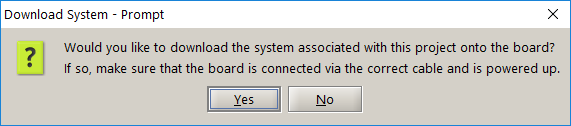
\includegraphics[scale=0.7]{figures/monitor_figure3.png}
		\caption{Pop-up window to download the system to the board.} 
		\label{fig:monitor_figure3}
	\end{figure}
	
	\item Click {\bf Actions > Compile \& Load} to compile the source code of your program. If it's your first time compiling the code, it will take a while because the Monitor Program will generate the necessary files for the API functions of SGDMA controllers. 
	
	\item Then click {\bf Actions > Continue} to start running the program on the board. You should see the message on the Monitor Program terminal screen as shown in Figure~\ref{fig:monitor_figure4}.
	
	\begin{figure}[H]
		\centering
		  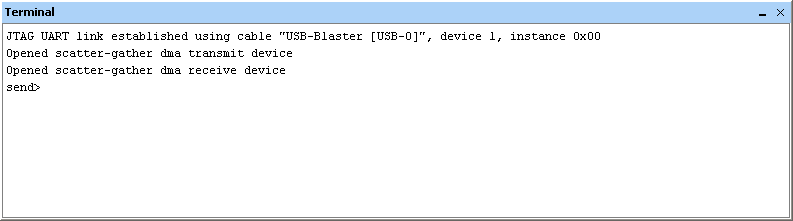
\includegraphics[scale=0.75]{figures/monitor_figure4.png}
		\caption{Running the application program by using the Monitor Program.} 
		\label{fig:monitor_figure4}
	\end{figure}	
	
	\item To make the demonstration program work properly, connect both Ethernet ports of the DE2-115 with an Ethernet cable. After connecting the ports, check the green LEDs besides the PHY chips to see in which mode the PHY chips are operating. Make sure the Triple-Speed Ethernet IP Core is operating in the same mode as the PHY chips. 
	
	\item Place the cursor in the terminal screen after the {\bf send>} label and type a message, then press the {\bf Enter} key to transmit the message. The message will be transmitted from the Ethernet1 port to the Ethernet0 port. Since the Ethernet0 port is set to perform a loopback, the message is transmitted back to the Ethernet1 port. Then, the message you type should be printed on the terminal screen after the label {\bf receive>}. An example is shown in Figure~\ref{fig:monitor_figure5}.

	\begin{figure}[H]
		\centering
		  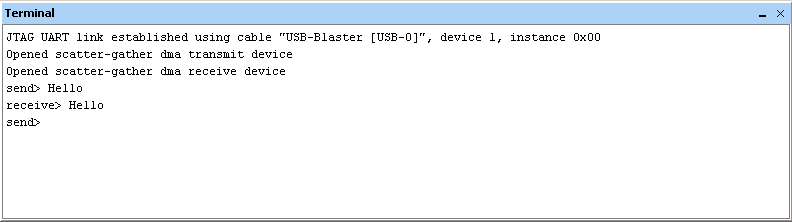
\includegraphics[scale=0.75]{figures/monitor_figure5.png}
		\caption{Sending messages.} 
		\label{fig:monitor_figure5}
	\end{figure}

\end{enumerate}

\newpage
\section{Concluding Remarks}
This tutorial shows how to build a Triple-Speed Ethernet system and run a simple application program on it. In most applications, using the Ethernet allows the system to communicate with any other device that supports Ethernet standard. While these details are beyond the scope of this tutorial, completing the tutorial provides the basic knowledge. If you are going to connect your system to some other devices, the next step should be to write software for the Nios II processor to handle the necessary protocols of higher layers.


% Copyright and Trademark

%\newcommand{\datePublished}{Mar 2022}

\newcommand{\versnum}{21.1} %version number quartus/AMP
\newcommand{\quartusname}{Quartus\textsuperscript{\textregistered} Prime}	
\newcommand{\textBar}{For \quartusname{} \versnum{}}
\newcommand{\thisyear}{2022 } %for copyright
\newcommand{\company}{FPGAcademy.org}
\newcommand{\longteamname}{FPGAcademy.org}
\newcommand{\teamname}{FPGAcademy}
\newcommand{\website}{FPGAcademy.org}

\newcommand{\productAcronym}{AMP}
\newcommand{\productNameShort}{Monitor Program}

\newcommand{\productNameMedTM}{Monitor Program}
\newcommand{\productNameMed}{Monitor Program}

%\newcommand{\headerLogoFilePath}[1]{#1/FPGAcademy.png}



%%%%%%%%%%%%%%%%%%%%%%%%%%%%%%%%%%%%%%%%
%%% FPGAcademy Copyright Information %%%
%%%%%%%%%%%%%%%%%%%%%%%%%%%%%%%%%%%%%%%%

%Always put the copyright on a new page (clear page), with some vertical space from top
\clearpage
\vspace{1in}

\noindent

Copyright {\copyright} FPGAcademy.org. All rights reserved. FPGAcademy and the FPGAcademy logo are trademarks of  FPGAcademy.org.  This document is being provided on an ``as-is'' basis and as an accommodation and therefore all warranties, representations or guarantees of any kind (whether express, implied or statutory) including, without limitation, warranties of merchantability, non-infringement, or fitness for a particular purpose, are specifically disclaimed.

%FPGAcademy assumes no responsibility or liability arising out of the application or use of any information,  product,  or  service  described  herein  except  as  expressly  agreed  to  in  writing  by  FPGAcademy.



**Other names and brands may be claimed as the property of others.




\end{document}
